\documentclass[11pt]{article}
\usepackage[parfill]{parskip}
\usepackage{graphicx}
\usepackage{wrapfig}
\usepackage{subcaption}
\usepackage[top=1in, bottom=1in, left=1in, right=1in]{geometry}
\bibliographystyle{plain}
\usepackage{amsmath}
\usepackage{amsfonts}
\usepackage{hyperref}
\usepackage{listings}
\usepackage{xcolor}

\usepackage{listings}
\usepackage{xcolor}
 
\definecolor{codegreen}{rgb}{0,0.6,0}
\definecolor{codegray}{rgb}{0.5,0.5,0.5}
\definecolor{codepurple}{rgb}{0.58,0,0.82}
\definecolor{backcolour}{rgb}{0.95,0.95,0.92}

\lstdefinestyle{mystyle}{
    backgroundcolor=\color{backcolour},   
    commentstyle=\color{codegreen},
    keywordstyle=\color{magenta},
    numberstyle=\tiny\color{codegray},
    stringstyle=\color{codepurple},
    basicstyle=\ttfamily\footnotesize,
    breakatwhitespace=false,         
    breaklines=true,                 
    captionpos=b,                    
    keepspaces=true,                 
    numbers=left,                    
    numbersep=5pt,                  
    showspaces=false,                
    showstringspaces=false,
    showtabs=false,                  
    tabsize=2
  }

 \lstdefinelanguage{Julia}%
  {morekeywords={abstract,break,case,catch,const,continue,do,else,elseif,%
      end,export,false,for,function,immutable,import,importall,if,in,%
      macro,module,otherwise,quote,return,switch,true,try,type,typealias,%
      using,while},%
   sensitive=true,%
   morecomment=[l]\#,%
   morecomment=[n]{\#=}{=\#},%
   morestring=[s]{"}{"},%
   morestring=[m]{'}{'},%
}[keywords,comments,strings]%
 
\lstset{style=mystyle}

%%%%%%%%%%%%%%%%%%%%%%%%%%%%%%%%%%%%%%%%%%%%%%%%%%%%%%%%%%%%%%%
\usepackage{fancyhdr}
\pagestyle{fancy}
%%% Please add the author's last names
\lhead{Galois TA2 AMIDOL}
\rhead{ASKE Milestone 6 Report}
%%% Please use \cfoot{} to remove page numbers
\cfoot{ }
\renewcommand{\headrulewidth}{0pt}
\renewcommand{\footrulewidth}{0pt}
%%%%%%%%%%%%%%%%%%%%%%%%%%%%%%%%%%%%%%%%%%%%%%%%%%%%%%%%%%%%%%&
\usepackage{amsthm}
 
\theoremstyle{definition}
\newtheorem{definition}{Definition}[section]

\colorlet{punct}{red!60!black}
\definecolor{background}{HTML}{EEEEEE}
\definecolor{delim}{RGB}{20,105,176}
\colorlet{numb}{magenta!60!black}

\usepackage{amsthm}

\newtheorem{mydef}{Definition}

\lstdefinelanguage{json}{
    basicstyle=\normalfont\ttfamily,
    numbers=left,
    numberstyle=\scriptsize,
    stepnumber=1,
    numbersep=8pt,
    showstringspaces=false,
    breaklines=true,
    frame=lines,
    backgroundcolor=\color{background},
    literate=
     *{0}{{{\color{numb}0}}}{1}
      {1}{{{\color{numb}1}}}{1}
      {2}{{{\color{numb}2}}}{1}
      {3}{{{\color{numb}3}}}{1}
      {4}{{{\color{numb}4}}}{1}
      {5}{{{\color{numb}5}}}{1}
      {6}{{{\color{numb}6}}}{1}
      {7}{{{\color{numb}7}}}{1}
      {8}{{{\color{numb}8}}}{1}
      {9}{{{\color{numb}9}}}{1}
      {:}{{{\color{punct}{:}}}}{1}
      {,}{{{\color{punct}{,}}}}{1}
      {\{}{{{\color{delim}{\{}}}}{1}
      {\}}{{{\color{delim}{\}}}}}{1}
      {[}{{{\color{delim}{[}}}}{1}
      {]}{{{\color{delim}{]}}}}{1},
}

\newcommand{\amidol}{\textsc{AMIDOL}}

\def\signed #1{{\leavevmode\unskip\nobreak\hfil\penalty50\hskip2em
  \hbox{}\nobreak\hfil(#1)%
  \parfillskip=0pt \finalhyphendemerits=0 \endgraf}}

\newsavebox\mybox
\newenvironment{aquote}[1]
  {\savebox\mybox{#1}\begin{quote}}
  {\signed{\usebox\mybox}\end{quote}}

\date{\vspace{-5ex}}
% Use this to get rid of the date

\usepackage{authblk}
\author[1]{Eric Davis}
\author[1]{Alec Theriault}
\author[1]{Ryan Wright}
\affil[1]{Galois, Inc}

%\setcounter{page}{0}



\title{May ASKE Milestone 7 Report for \amidol{}}

\begin{document}
\maketitle
\vspace{10pt}

\section{Introduction}

In this report we discuss recent extensions to \amidol{}'s framework
which seek to extend \amidol{}'s Abstract Knowledge Layer and
Formulation and Palette generation capabilities, and briefly discuss
extensions to \amidol{}'s ability to work with additional intermediate
representations at the Structured Knowledge Layer, and support for
additional backends for its Executable Knowledge Layer.

\section{Formulations}

\amidol{}'s Abstract Knowledge Layer focuses on the representation,
manipulation, and extension of problem formulations as part of the
metamodeling process.

\begin{definition}{Formulation}
  A formulation is a high-level domain model which represents and
  encodes semantic domain knowledge about a complex system.
  Formulations are the model-stack equivalent of a high level
  language and should focus on being accessible to domain scientists.
  While formal semantics may be implied by a formulation, the primary
  point of formulating a model is not writing down executable code or
  mathematical representations.  It is
  writing down assumptions and knowledge which can, at a later stage,
  be used to infer these properties of a model.

  Formulations should be represented in a form that is close to
  natural language, or natural representations, such as diagrams, used
  by domain scientists.

  Formulations define the Abstract Knowledge Layer of the modeling stack.
\end{definition}

The primary mechanism used for formulations in \amidol{} are Visual
Domain Specific Ontological Languages (VDSOLs).  VDSOLs attempt to
leverage the semi-formal diagrams domain scientists use when
describing and documenting systems; pairing them with formal
mathematical and executable meaning.  To accomplish this, a VDSOL is defined by
a Formulation Palette,

\begin{definition}{Formulation Palette}
  A formulation palette is a set $P = \{ p_0, p_1, \ldots\}$ of
  palette elements which can be used to construct a semi-formal
  diagram with underlying mathematical and executable meaning.
\end{definition}

Palettes form the core of the definition of a VDSOL and consist of
the valid symbols which can be used to instantiate concrete occurances
of a given palette element.

\begin{definition}{Palette Element}
  A palette element is a type which can be instantiated in a
  formulation as a concrete occurance of the element.  These instance
  elements must have unique names, and can be connected with arcs to
  define structured co-spans of instance elements which can be
  compiled into \amidol{}'s intermediate representation, providing
  formal mathematical meaning for a diagram expressed in a VDSOL.

  A palette element is defined by the combination of a palette
  template $T$, and a definition in \amidol{}'s intermediate
  representation $R$ into the tuple $(T,R)$

  An instance element is a palette element, combined with a unique
  identifier $N$ and a set of parameters and constants $C$, $(T, R, N,
  C)$.  The set of parameters and constants are used to override
  generic parameters and constants within a palette element,
  specializing it to a particular modeling case where necessary.
\end{definition}

Palette templates are abstract palette elements which have recently
been added to \amidol{} in order to support palette extenstion, both
automatically and manually.

\begin{definition}{Palette Template}
  A palette template is a category defined by an input set, output
  set, and measure set, over an unknown or undefined \amidol{} IR.
  Palette templates are essentially container categories for
  compatible \amidol{} IR models whose input and output cardinality
  and typing match, making them interchangable.
\end{definition}

Palette templates cannot be instantiated as a concrete instance
element, but they can be subclassed by a palette element.  Much like
abstract classes or methods in object oriented programming, palette
templates lack \emph{implementation}, in this case a paired IR representation.

A Formulation in \amidol{} is a set of palette element instances
composed together by a set of relations, $A \rightarrow B$ such that
for the output cardinality of $A$ and the input cardinality of $B$ are
the same, and have compatible types.  Type relations allow
restrictions on model composition which are richer than input/output
cardinality; such as that used by all current \amidol{} palettes which
states if $A$ is a noun, $B$ must be a verb, and if $A$ is a verb, $B$
must be a noun.  Further restrictions could be used to apply types to
individual inputs or outputs to restrict their composability to.

\subsection{Formulation Paradigm}

The process of model formulation in \amidol{} seeks to allow domain
experts to construct meta-models in a novel way, using VDSOLs.  These
VDSOLs utilize an
underlying intermediate abstract representation to give formal meaning
to the intuitive process diagrams scientists and domain experts
normally create.  The intention is to remove the burden of having to
code models explicitly, and enable domain experts to build models of
complex systems which are easier to maintain, validate, and verify,
and avoid common pitfalls of monolithic and hand-coded
implementations.

While to date these formulations have all been through the use of
diagrams, we are extending \amidol{} to support other types of formal
languages that are natural for certain domains.

\subsection{Formulation Languages}

To explore other types of visual languages and diagrams, we are
extending \amidol{} to support systems of stochastic chemical
equations via standard notations for networks of chemical reactions of
the form \[A +B \overset{\beta}{\rightarrow} C\] which is interpreted
as ``a molecule of $A$ combines with a molecule of $B$ to form a
molecule of $C$ with propensity $\beta$''.  We use the following
formal grammar to represent stochastic chemical equations in \amidol{}
as a formulation:

\lstinputlisting[caption=Stochastic Chemical Equation
Grammar]{equation.lark}

\amidol{} is capable of reading networks of chemical reactions, like
the following:

\begin{lstlisting}[caption=Example Stochastic Chemical Equation]
1.0,      A       -> B
2.0,      A + B <--> C + D
3.0, 4.0, A + B <--> C + D
\end{lstlisting}

and generating an abstract syntax tree like that shown in Figure
\ref{Fig:Reaction}.  This abstract syntax tree can then be used to
generate a model in the \amidol{} IR, representing each reactant with
a state variable, and constructing events from the identified equation
nodes.

\begin{figure}
  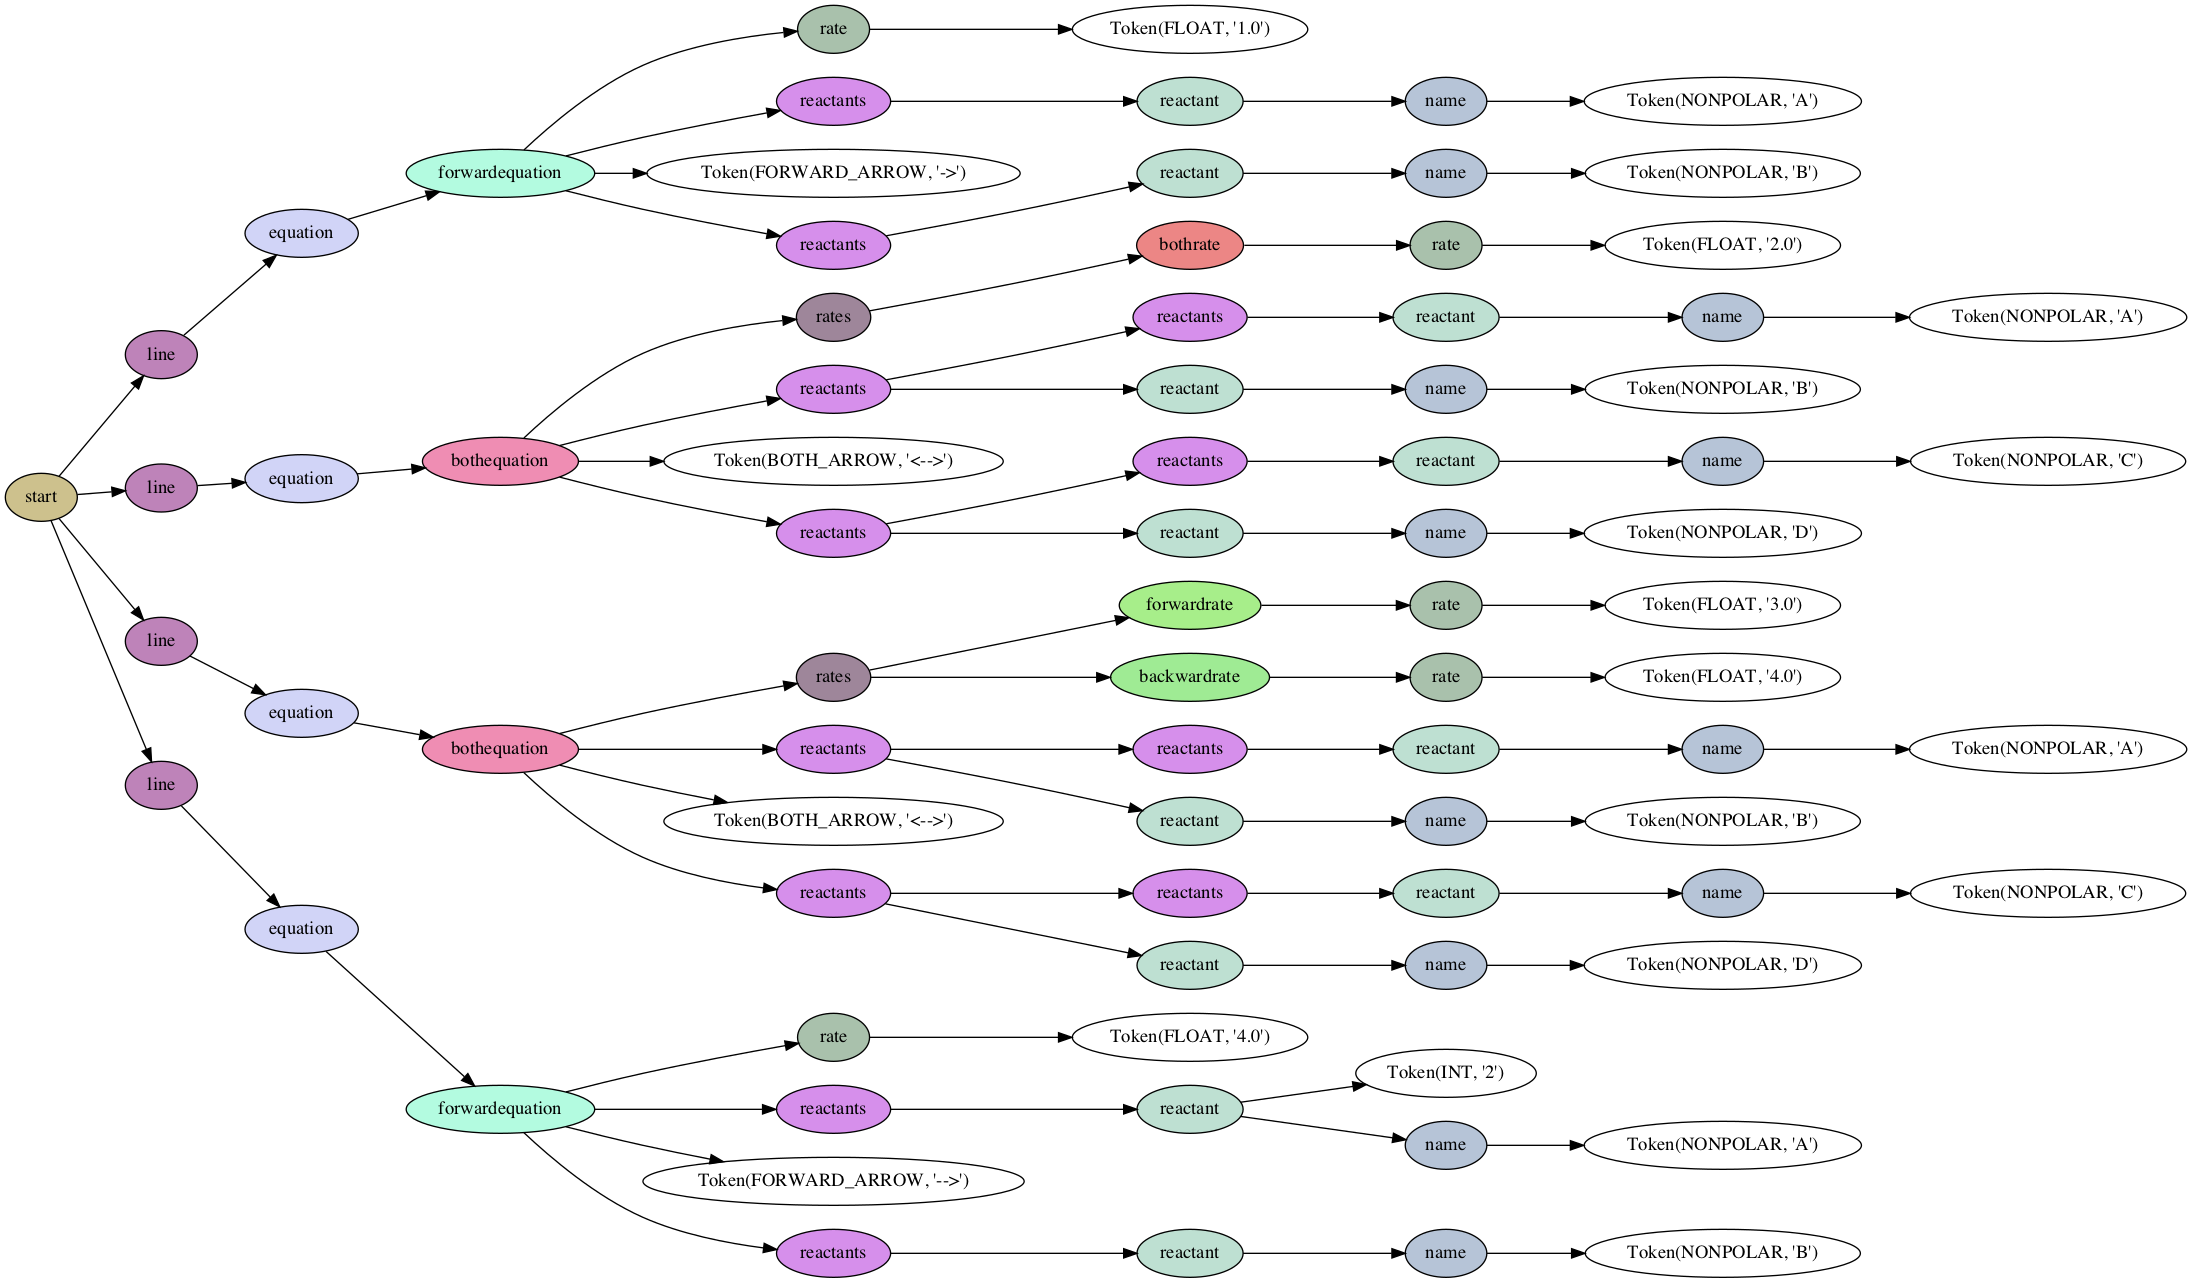
\includegraphics[width=\textwidth]{tree.png}
  \caption{Example Parse Tree from Stochastic Chemical Grammar}
  \label{Fig:Reaction}
\end{figure}

While designed to test the expressive capability of \amidol{}'s
Abstract Knowledge Layer in representing chemical equations, it can
also be used to represent other models, like the SIR model, as
follows:

\begin{lstlisting}[caption=Example Stochastic Chemical Equation]
beta / (S + I + R), S + I --> I
gamma,              I --> R
\end{lstlisting}

\section{Formulations from Models}

In order to support a joint demo with GTRI and the University of
Arizona, and the Knowledge Extraction workflow of moving up the stack,
we have also been developing methods which allow
us to automatically generate formulations in a visual language from
models at the Structured Knowledge Layer.  To support this, we have
constructed a new module for \amidol{} which is able to translate
Julia abstract syntax trees, like that shown in Figure \ref{Fig:JuliaAST}, into
\amidol{}'s IR.  These models are combined with grounding information
to perform the novel process of Formulation Inference in \amidol{}.

\begin{figure}
  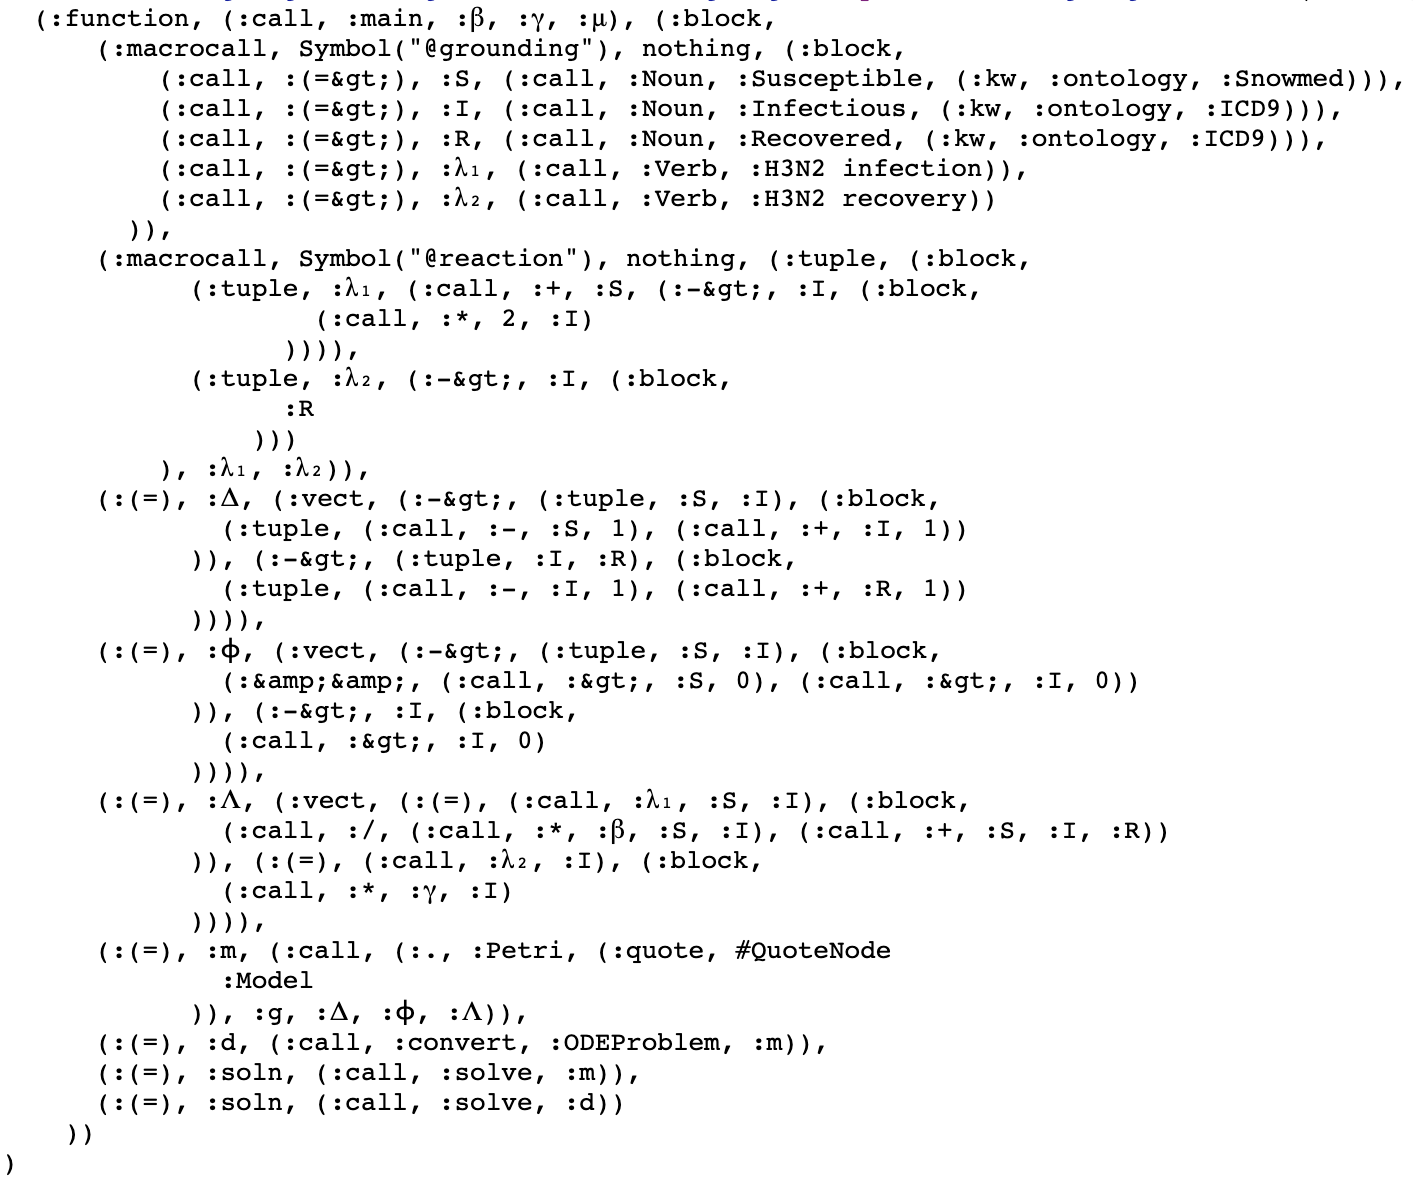
\includegraphics[width=\textwidth]{AST.png}
  \caption{Julia Abstract Syntact Tree for SIR Model}
  \label{Fig:JuliaAST}
\end{figure}

\subsection{Formulation Inference}

Formulation Inference is a formal procedure in \amidol{} for
automatically generating new palette elements from existing palette
templates, using an ontology of domain specific terms.

\begin{figure}
  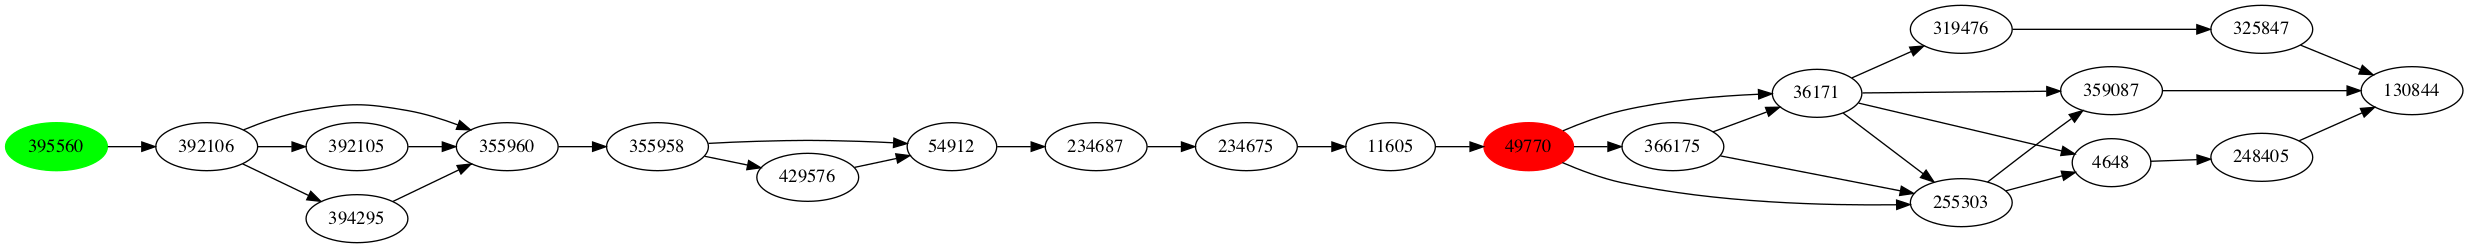
\includegraphics[width=\textwidth]{H3N2vmap.png}
  \caption{Ontology search for viral template from grounding
    ``Influenza A virus subtype H3N2v''}
  \label{Fig:ontology1}
\end{figure}

Figure \ref{Fig:ontology1} shows a subset of the SNOMED CT ontology,
representing elements of the ontology with nodes labeled with their
SCTID.  In this example, the green node represents the term
``Influenza A virus subtype H3N2v'' while the red node represents the
term ``Virus (organism)''.  Formulation inference assumes the
existance of an annotated ontology, with nodes containing palette
templates as annotations.  In this example the ``Virus (organism)''
node has been annotated with the palette template for a viral
infection verb.

For this example, assume we have a Julia AST representing the
infection process, which has been transformed into \amidol{}'s IR,
along with the attached grounding ``Influenza A virus subtype
H3N2v''.  Formulation inference executes a search on a specified
ontology, in this case SNOMED CT, and walks the parent relationships
from those nodes which match the grounding, searching for a palette
template.  If a palette template is found, we check the category of
the template against an inferred category from the IR representation
of our code by constructing a \emph{model dependency graph}.

\begin{definition}{Model Dependency Graph}
  A model dependency graph of a model $M$ is defined as a labeled
  graph $G_M = (V,A,L)$ where $V$ is the set of vertices composed of
  three subsets $V_S \cup V_E \cup V_{\Theta}$, $A$ is a set of arcs
  connecting two vertices such that arcs connect elements of the
  subset $V_S$ to $V_E$, or vice versa, or connect an element of
  $V_{\Theta}$ to $V_S \cup V_E$, and $L$ is a set of labels applied
  to elements of $A$ from the set $\{\Phi, \Lambda, \Delta,
  \Theta\}$.  The model dependence graph contains $v_i \in V_S$ for
  every state variable in the model, $v_j \in V_E$ for each event
  in the model, and $v_k \in V_{\Theta}$ for each measure defined in
  the model.

  Arcs in $A$ are defined such that, if an event $e_j$ has enabling
  conditions that depend on state $s_i$, an arc labeled $\Phi$ exists
  from $v_i \rightarrow v_j$; if an event $e_j$ has a state dependent
  rate defined in terms of $s_i$, an arc labeled $\Lambda$ exists
  from $v_i \rightarrow v_j$; if an event $e_j$ has a state transition
  function defined in terms of $s_i$ and whose firing results in $s_i'
  < s_i$, an arc labeled $\Delta$ exists from $v_i \rightarrow v_j$
  and if the firing results in $s_i' > s_i$, an arc labeled $\Delta$
  exists from $v_j \rightarrow v_i$.  Finally if a measure $\Theta_k$
  exists and is defined over $s_i$, an arc labeled $\Theta$ exists
  from $v_k \rightarrow v_i$, and if the measure is defined over
  $e_j$, an arc labeled $\Theta$ exists
  from $v_k \rightarrow v_j$.
\end{definition}

The model dependence graph is used to infer the category of a model,
and checked against any template found in the ontology search.  On a
successful matching to a template, the IR is used to infer a new
palette element which is added to the VDSOL palette, and can be
instantiated into new instance elements.

If a template is not found, a generic template is created from the
inferred category, and flagged
for user attention and resolution.

\section{The SNOMED Ontologies}

In order to support our goals for the demo, and \amidol{}'s new
formulation inference capabilities, we have implemented an ontology
ingestion pipeline for \amidol{}, and uploaded the SNOMED CT
ontology.  The SNOMED ontology consists of 466,612 concepts organized
as a directed acyclic graph, with parent/child relationships
represented.  Terms in the ontology have a maximum of 3,762 children,
each, and 36 parents.  We annotated this ontology with palette
templates for the SIR model palette.

\section{Examples}

The following examples demonstrate the behavior of \amidol{} when
performing palette inference from grounding.  In all of the following
examples, our goal was to find the palette template annotated at the
node for ``Virus (organism)''.  Figure
\ref{Fig:H1N1Grounding} shows the process of ontology search for a
template beginning with the grounding ``Influenza A (H1N1)''.  Each
green node represents a separate matching term, using substring
matching.  \amidol{} proceeded to follow all parent relationships, and
displayed all annotated nodes in red, successfully recovering the
palette template.

\begin{figure}
  \begin{center}
    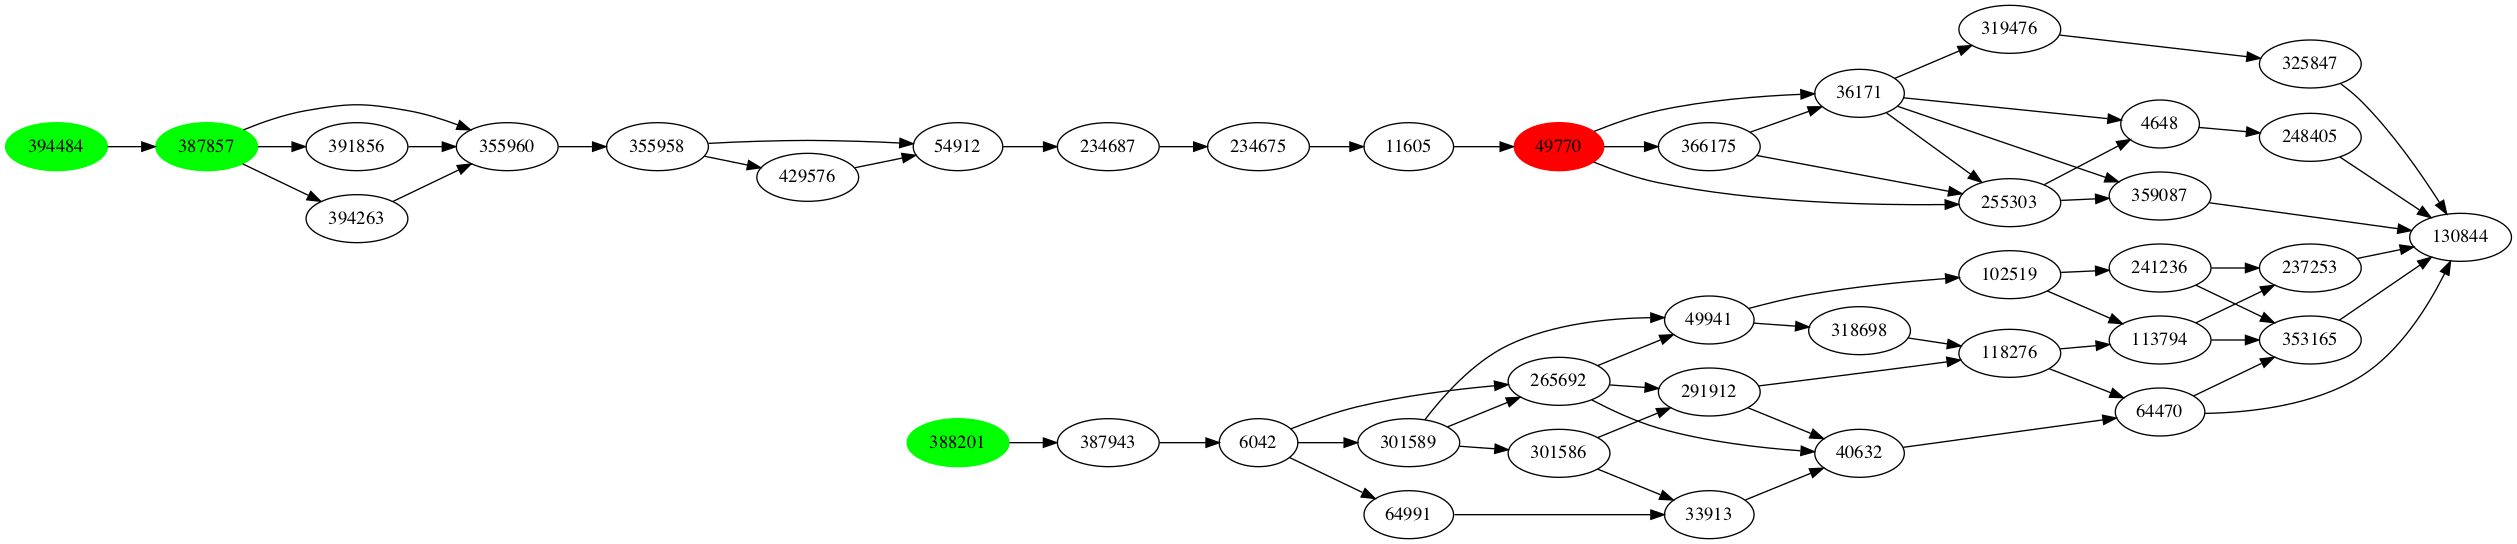
\includegraphics[width=\textwidth]{H1N1.png}
  \end{center}
  \caption{Ontology search for viral template from grounding
    ``Influenza A (H1N1)''}
  \label{Fig:H1N1Grounding}
\end{figure}

Figure \ref{Fig:H3N2Grounding} shows the results from searching on the
grounding ``H3N2''.  Note the results are quite different than those
presented in Figure \ref{Fig:ontology1}, as far more nodes matched the
term search, requiring a larger search of the ontology to find
potential palette templates.

\begin{figure}
  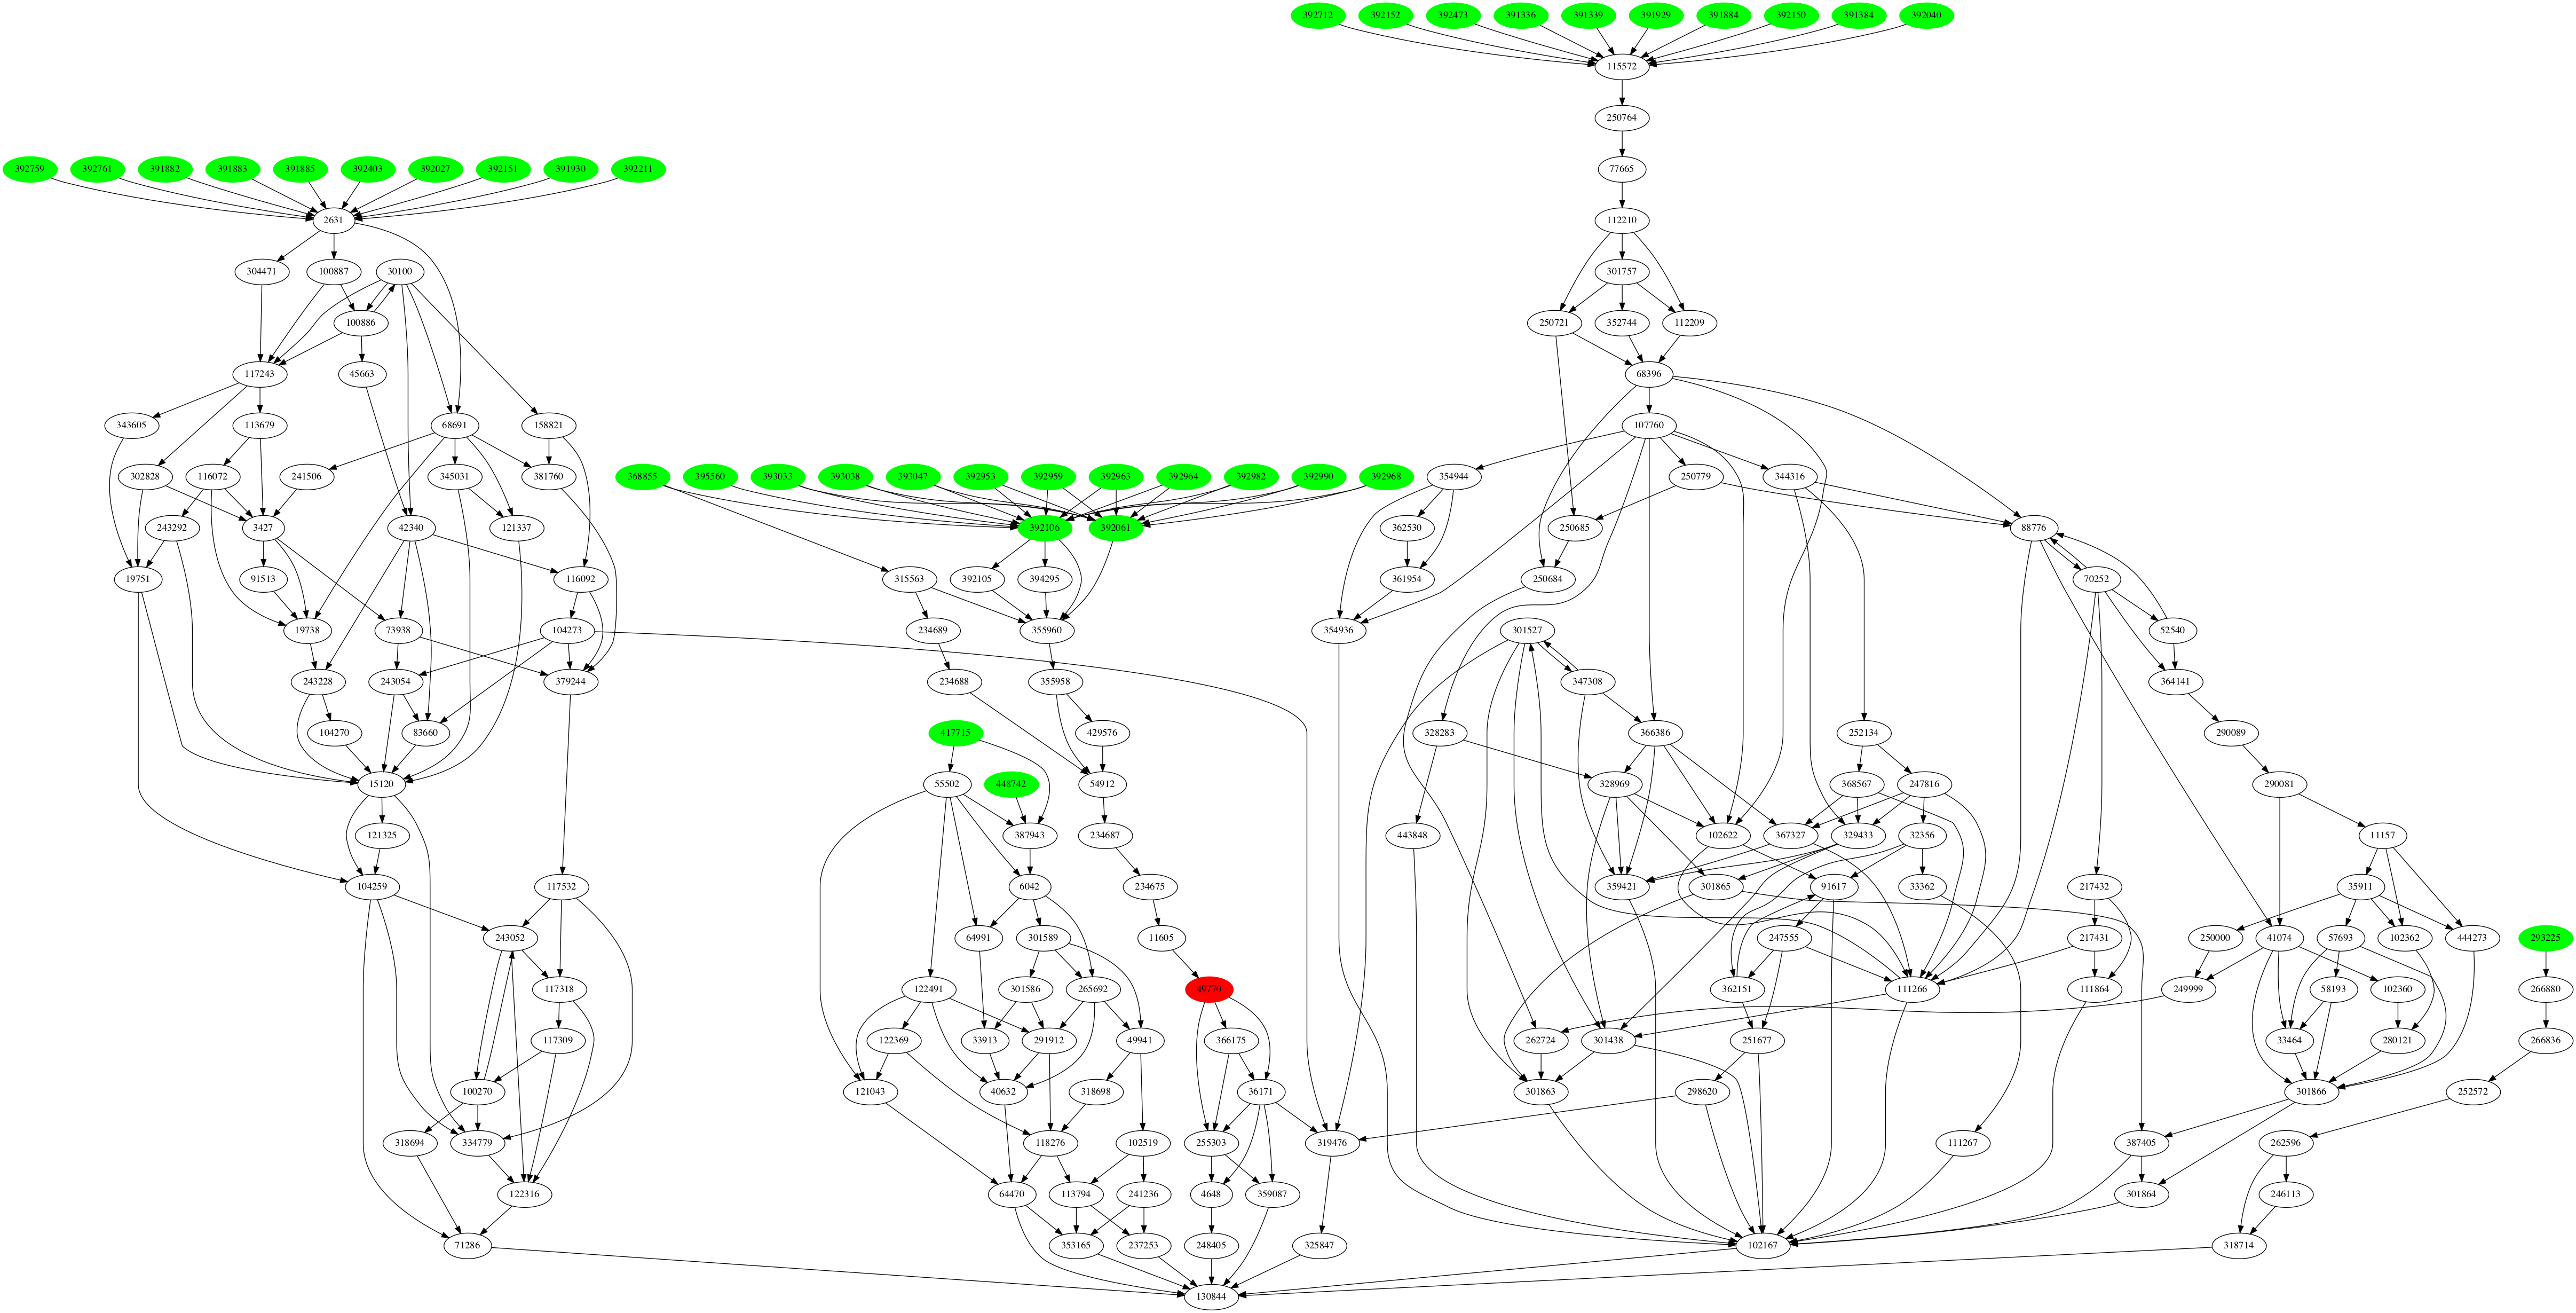
\includegraphics[width=\textwidth]{H3N2map.png}
  \caption{Ontology search for viral template from grounding ``H3N2''}
  \label{Fig:H3N2Grounding}
\end{figure}

Figure \ref{EbolaGrounding} shows the same process for the grounding
``Ebola'', also recovering the viral template.

\begin{figure}
  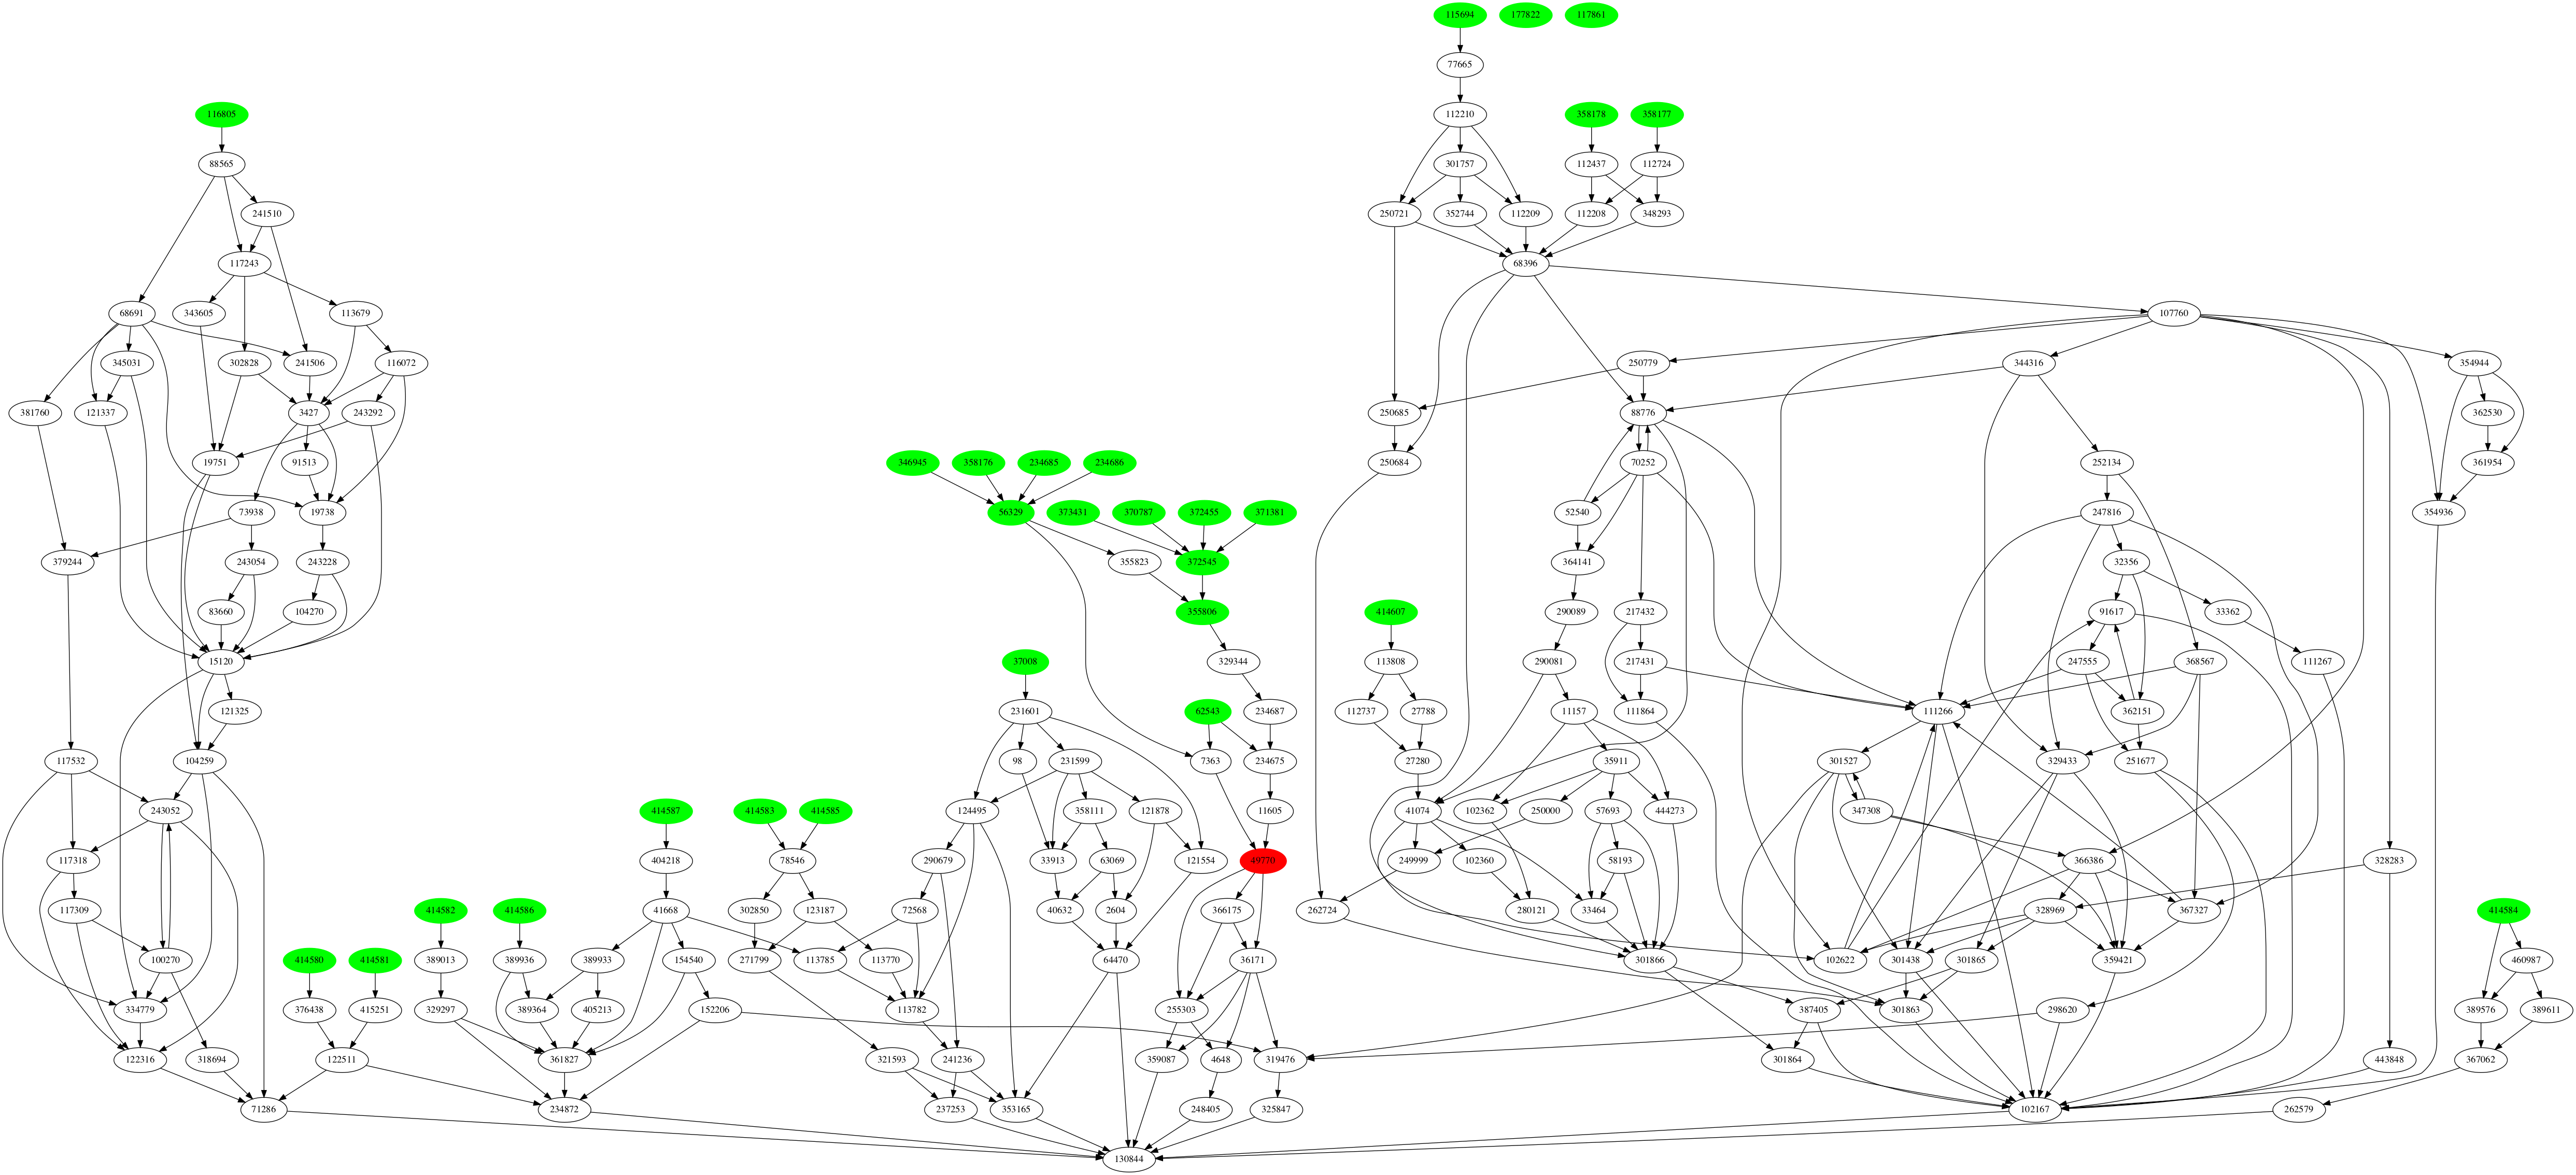
\includegraphics[width=\textwidth]{Ebolamap.png}
  \caption{Ontology search for viral template from grounding
    ``Ebola''}
  \label{Fig:EbolaGrounding}
\end{figure}

Our initial experiments have been successful, and suggest the
suitability for this algorithm for formulation inference using
human-in-the-loop teaming with \amidol{}.

\section{Other Recent AMIDOL Extensions}

In addition to the major extensions described above, we have also
extended \amidol{} to support new back-end solvers for the Executable
Knowledge Layer, including agent-based models in Julia and Python, and
ODE-based solvers in Julia.

\section{Resources, web sites, etc.}

The current \amidol{} source code, including example models and documentation, is available at the \amidol{} Github site \url{https://github.com/GaloisInc/AMIDOL}.

\bibliography{AMIDOL-MWS}

\end{document}
